\section{Low-Temperature Transport Measurements in a Strong Magnetic Field}
\label{sec:expsetup:magnet}

\subsection{High Field Magnets and Cryostats}\label{magnet}

The main in-house magnets we use are the 14 Tesla superconducting magnet from Oxford Instruments, the 15 Tesla superconducting magnet from American Magnetics, and the 9 Tesla Physical Property Measurement System (PPMS) from Quantum Design. Besides, we also use the 35 Tesla Resistive Magnet, the 45 Tesla Hybrid Magnet, and the 65 Tesla Pulse Field Magnet at National High Magnetic Field Laboratory (NHMFL) to study our samples at high fields. The high field data can provide us important information such as low Landau levels and possible new phases.


\begin{figure}[!htbp]
  \begin{center}
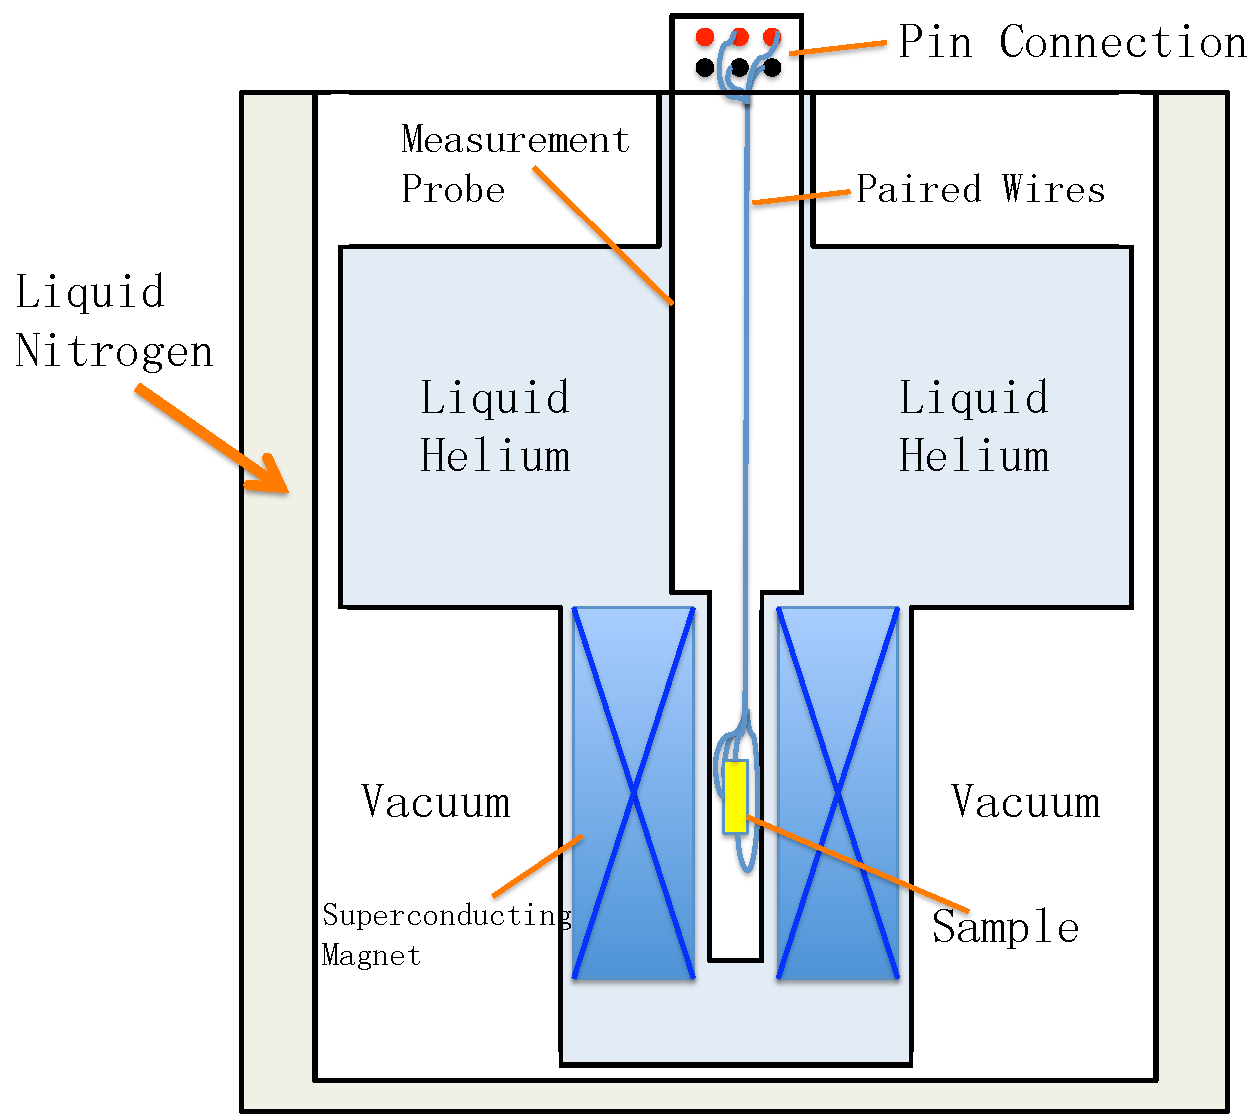
\includegraphics[width=0.8\linewidth]{ch-expsetup/figures/Magnet14T.pdf}
\caption{\label{Magnet14T}
A sketch of a typical in-house superconducting magnet with a measurement probe inside.}
  \end{center}
\end{figure}

Our in-house magnets are similar in their structures as shown in Fig. \ref{Magnet14T}. Each magnet has a dense coil made out of superconducting materials. The coil, with a bore for the measurement probe, is immersed by liquid helium in a dewar with a vacuum jacket. Outside the vacuum jacket, there is a liquid nitrogen jacket in order to reduce the thermal radiation from the helium container. The coil has a critical temperature higher than 4.2 K, and thus the coil will stay in the superconducting state when the current is flowing inside. The current is driven by an outside power supply. 

\subsection{Transport Measurement}\label{transport}

%talk about Sample Sample method
To make ohmic contacts to the samples, we typically use the silver paint from Dupont and thin gold wires to connect the sample to the measurement pads on the sample stage. To measure the magnetoresistance at tilted magnetic fields, we leverage our home-made rotation probe and the rotation probe that accompanies PPMS to rotate the sample in a magnetic field. Our home-made rotation probe has a Hall probe to tell the angle relative to the direction of the magnetic field. It can reach a temperature as low as 4.5 K, while PPMS's rotation probe can get to 2 K. To measure the transport property below 4 K, we use the He3 inserts from Oxford, Janis and IceOxford to to attain 0.3 K. Besides, NHMFL provides measurement inserts for both 4K-above and 4K-below transport measurements in the high-field experiments. To stabilize the temperature, we use the Lakeshore 340 temperature controller to adjust the heating power on the sample stage. 

The resistivity transport measurements were accomplished in different ways, such as by the lock-in technique and the delta-mode method. In the PPMS, we use the DC Resistivity mode (which is actually a delta mode) to measure the magnetoresistance. To measure the sample resistance in our in-house superconducting magnet, we typically use the SR830 Lock-in Amplifier from Stanford Research to implement the lock-in measurement, or use Keithley's 6221 current source and 2182A nano voltmeter for the delta-mode method. The choice depends on the sample's resistance as well as its contact resistance. Besides, the current through the sample is carefully chosen so that it has a large signal-to-noise ratio and does not increase the sample temperature. 

The Hall measurement is conducted in a way similar to the resistance measurement. But one noticeable detail is the method to measure the temperature dependence of the Hall coefficient. Here we implement the reciprocal technique set up by Sample et.al.\cite{Sample1987}. This method leverages the reciprocal theorem in electrodynamics so that the magnetic field does not need to be flipped during the Hall measurement. 

The main idea in Sample's work\cite{Sample1987} is as the following. Suppose there is a sample with four contact leads labeled as 1, 2, 3 and 4 respectively. In a magnetic field pointing to the positive direction, we first measure the resistance $R_{12, 34} (+B)$ by sending a current through leads 1 and 2, while measuring the voltage on leads 3 and 4. When we reverse the field direction, $R_{34, 12} (-B)$ denotes the resistance measured across the leads 1 and 2 with the current flowing through the leads 3 and 4. And the reciprocal theorem gives $R_{12, 34} (+B) = R_{34, 12} (-B)$. Therefore, we can also obtain $R_{12, 34} (-B) = R_{34, 12} (+B)$. In a Hall measurement, we normally need both $R_{12, 34} (+B)$ and $R_{12, 34} (-B)$ to calculate the Hall signal by $R_{yx} (B) = (R_{12, 34} (+B) - R_{12, 34} (-B))/2$ so that the extra contribution from the longitudinal resistance can be neutralized. But this conventional way also requires a change of the field direction, which usually takes a long time. Here we replace $R_{12, 34} (-B)$ with $R_{34, 12} (+B)$, and obtain $R_{yx} (B) = (R_{12, 34} (+B) - R_{34, 12} (+B))/2$. As a result, we do not need to flip the magnetic field. Instead, we need to switch the current and voltage leads, which can be done quickly with an electric relay switch. Using this method, we are able to switch the the current and voltage leads at each temperature and then measure the Hall coefficient v.s. temperature curve in a short time. 
